\begin{figure}[p]\centering
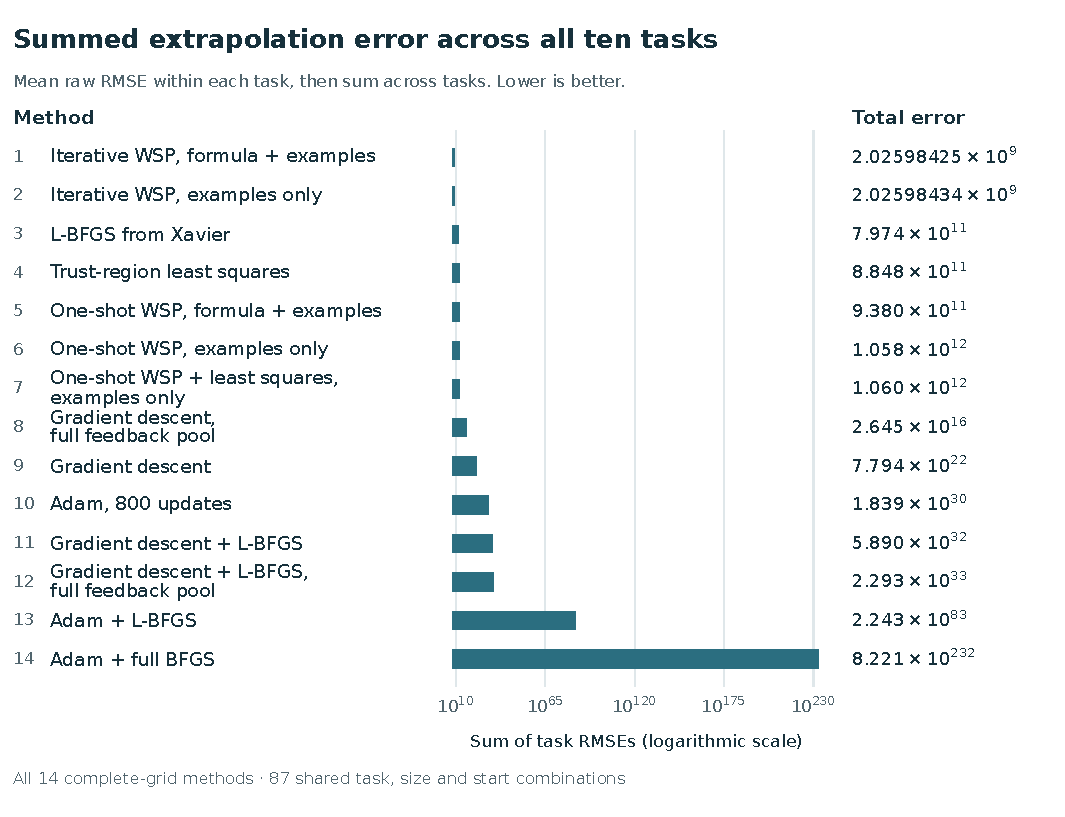
\includegraphics[width=\linewidth]{holistic_full_range.pdf}
\caption{The full range of summed raw extrapolation errors. Each method is evaluated on the same 87 task, architecture and start combinations. For each task, we average raw root mean squared error (RMSE) across its tested sizes and three starts, then sum those ten task values. Each task contributes one mean; output scales are not normalized. Ranks use unrounded totals. The two iterative WSP totals agree to six significant figures. The full feedback-pool controls use additional labels, and WSP followed by least squares receives an additional numerical stage. Adam means adaptive moment estimation; BFGS means Broyden--Fletcher--Goldfarb--Shanno. Large-magnitude targets and individual divergent runs strongly affect this raw sum. Fibonacci contributes more than 99.8\% of examples-only one-shot WSP's total. Positive self-power contributes about 78.1\% of its iterative counterpart's total.}\label{fig:holisticfull}
\end{figure}
